% Generated by book/tools/notebook_to_tex.py. Do not edit by hand.

\chapter[BERT 이진 분류: Softmax (CE)]{BERT 이진 분류: Softmax (CE)}

\label{ch:11}

\markboth{BERT 이진 분류: Softmax (CE)}{BERT 이진 분류: Softmax (CE)}

\chaptermeta{11_bert_binary_softmax/11_bert_binary_softmax.ipynb}{https://colab.research.google.com/github/yoon-gu/neuqes-101/blob/master/11_bert_binary_softmax/11_bert_binary_softmax.ipynb}{num\_labels=2, softmax, CrossEntropyLoss 표준 BERT 분류 방식}



\index{1BERT binary softmax@BERT binary softmax}

\index{1softmax@softmax}

\index{1CrossEntropyLoss@CrossEntropyLoss}

\index{1num labels 2@num\_labels=2}

\index{1single label classification@single\_label\_classification}

\index{1id2label@id2label}

\index{1label2id@label2id}

\index{1logit difference@logit difference}

\index{1prediction agreement@prediction agreement}

\index{0소프트맥스@소프트맥스}

\index{0교차 엔트로피@교차 엔트로피}

\index{0라벨 매핑@라벨 매핑}

\index{0로짓 차이@로짓 차이}

\index{0예측 일치율@예측 일치율}

\index{0이진 분류 동등성@이진 분류 동등성}

\index{1problem type single label classification@problem\_type="single\_label\_classification"}

\index{1stable softmax@stable softmax}

\index{1exp x max@exp(x - max)}

\index{1scatter plot@scatter plot}

\index{1correlation@correlation}

\index{1four quadrant analysis@four-quadrant analysis}

\index{0표준 분류 셋업@표준 분류 셋업}

\index{0안정 소프트맥스@안정 소프트맥스}

\index{0상관계수@상관계수}

\index{04분면 분석@4분면 분석}



\section{변화추적표}

\begin{booktable}{11장 변화추적표}{tab:ch11-01}
\begin{adjustbox}{max width=\textwidth}
\begin{tabular}{@{}lllllll@{}}
\toprule
Ch & 모델 & 토크나이저 & 데이터 & Output Head & Activation & Loss \\
\midrule

3 & \inlinecode{LogisticRegression()} & \inlinecode{TfidfVectorizer()} & Yelp 이진화 & (1차원) & sigmoid & \inlinecode{BCEWithLogitsLoss} \\
4 & \inlinecode{LogisticRegression(multi\_class="multinomial")} & \inlinecode{TfidfVectorizer()} & Yelp 이진화 (\ref{ch:03}장과 동일) & (2차원) & softmax & \inlinecode{CrossEntropyLoss} \\
9 & DistilBERT 파인튜닝 & \inlinecode{AutoTokenizer.from\_pretrained(...)} & Yelp (별점 1-5) & \inlinecode{Linear(H,\ 1)} & 없음 & \inlinecode{MSELoss} \\
10 & DistilBERT 파인튜닝 & 같음 & Yelp 이진화 & \inlinecode{Linear(H,\ 1)} & sigmoid & \inlinecode{BCEWithLogitsLoss} \\
\textbf{11 ← 여기} & DistilBERT 파인튜닝 & 같음 & Yelp 이진화 (\ref{ch:10}장과 동일) & \textbf{\inlinecode{Linear(H,\ 2)}} & \textbf{softmax} & \textbf{\inlinecode{CrossEntropyLoss}} \\
12 (다음) & DistilBERT 파인튜닝 & 같음 & Yelp 5클래스 & \inlinecode{Linear(H,\ 5)} & softmax & \inlinecode{CrossEntropyLoss} \\
\bottomrule
\end{tabular}
\end{adjustbox}
\end{booktable}

전체 20장 표는 \href{https://github.com/yoon-gu/neuqes-101\#챕터별-변화추적표}{루트 README.md}를 참고하세요.



\section{변경점: \ref{ch:10}장 대비}

\begin{booktable}{11장 변경점 요약}{tab:ch11-02}
\begin{adjustbox}{max width=\textwidth}
\begin{tabular}{@{}lll@{}}
\toprule
축 & \ref{ch:10}장 (방식 A) & \ref{ch:11}장 (방식 B) \\
\midrule

\inlinecode{num\_labels} & 1 & \textbf{2} \\
\inlinecode{problem\_type} & \inlinecode{"multi\_label\_classification"} & \textbf{\inlinecode{"single\_label\_classification"}} ← BERT 표준 분류 \\
Activation & sigmoid & \textbf{softmax} \\
Loss & \inlinecode{BCEWithLogitsLoss} & \textbf{\inlinecode{CrossEntropyLoss}} \\
라벨 형식 & float \texttt{{[}0.0{]}} / \texttt{{[}1.0{]}} (multi-hot 1차원) & \textbf{int \inlinecode{0} / \inlinecode{1}} (스칼라 인덱스) \\
모델 출력 shape & \inlinecode{(B,\ 1)} & \textbf{\inlinecode{(B,\ 2)}} \\
데이터 / 모델 본체 / hyperparams & (변동 없음) & (그대로) \\
\bottomrule
\end{tabular}
\end{adjustbox}
\end{booktable}

\begin{quote}
\textbf{정확히 하나의 축만 바뀝니다} --- 이 장에서 변하는 건 \emph{Loss 축} (BCE → CE)이고, 그에 따라가는 부수적 변화(num\_labels, activation, 라벨 형식)는 모두 \emph{같은 축의 일관된 표현 변경} 입니다. 데이터·모델·학습 hyperparams는 \ref{ch:10}장과 \emph{완전히 동일} 하게 유지해야 마지막 비교가 의미가 있습니다.
\end{quote}

\subsection{두 방식의 동등성}

방식 A의 확률: \(\hat p_A = \sigma(z)\) --- \emph{1차원 logit} \(z\).

방식 B의 확률: \(\hat p_B = \mathrm{softmax}(z_0, z_1)[1] = \dfrac{e^{z_1}}{e^{z_0} + e^{z_1}} = \dfrac{1}{1 + e^{-(z_1 - z_0)}} = \sigma(z_1 - z_0)\).

→ \textbf{\(z_A \equiv z_1 - z_0\)} 으로 두면 두 방식이 수학적으로 같은 함수입니다. 학습된 가중치는 다른 경로로 수렴하지만, \emph{최종 확률} 은 거의 같아야 합니다 (\ref{ch:04}장에서 sklearn으로 봤던 그 동등성).



\section{\texorpdfstring{손실 노트}{손실 노트}}

\begin{equation}
\label{eq:ch11-01}
L = -\frac{1}{N}\sum_{i=1}^{N}\log \hat p_{i, y_i} \quad\text{where}\quad \hat p_{i,k} = \dfrac{e^{z_{i,k}}}{\sum_{j} e^{z_{i,j}}}
\end{equation}

식~\eqref{eq:ch11-01}은 이 절에서 사용하는 핵심 관계를 정리한 것입니다.

이 장에서 새로운 점은 없고 --- \ref{ch:04}·\ref{ch:05}장에서 이미 다 익혔습니다. \emph{BERT} 라는 컨텍스트로 옮겨 쓸 뿐입니다.

\textbf{숫자로 감 잡기 (binary, K=2)} --- 정답이 클래스 1, logits를 \((z_0, z_1)\) 로 두면:

\begin{booktable}{11장 손실 노트 표}{tab:ch11-03}
\begin{adjustbox}{max width=\textwidth}
\begin{tabular}{@{}lll@{}}
\toprule
logits \((z_0, z_1)\) & softmax → \((p_0, p_1)\) & 정답=1일 때 손실 \(-\log p_1\) \\
\midrule

\((0, 0)\) & \((0.5, 0.5)\) & 0.693 \\
\((0, 2)\) & \((0.119, 0.881)\) & 0.127 \\
\((0, 5)\) & \((0.007, 0.993)\) & 0.007 \\
\((0, -2)\) & \((0.881, 0.119)\) & \textbf{2.127} \\
\bottomrule
\end{tabular}
\end{adjustbox}
\end{booktable}

\(z_1 - z_0\) 의 크기가 정답 클래스 쪽으로 클수록 손실이 작아집니다. \textbf{방식 A의 \(z\) 와 정확히 같은 신호}: \(\sigma(z_1 - z_0) = p_1\) 가 1에 가까우면 손실이 작음.

\textbf{\inlinecode{CrossEntropyLoss} 의 안정성} --- PyTorch \inlinecode{nn.CrossEntropyLoss} 는 내부적으로 \emph{log-softmax + NLL} 로 구현되어 있어 \inlinecode{BCEWithLogitsLoss} 와 동일하게 \textbf{logit에서 직접 계산} (softmax를 따로 적용하지 않음). 두 loss 모두 “raw logit 받아서 안정적인 log-sum-exp 트릭으로 처리” 라는 점이 같습니다.



\section{토크나이저 노트}

\ref{ch:10}장과 동일한 \inlinecode{distilbert-base-uncased} WordPiece 토크나이저, 동일한 max\_length=128. 토크나이저 단계는 그대로지만 \textbf{\inlinecode{tokenize\_fn} 안에서 라벨을 \texttt{{[}float(b){]}} 가 아닌 \inlinecode{int(b)} 로 둡니다} --- 이게 이 장의 데이터 측 유일한 변경.



\Needspace{8\baselineskip}
\begin{lstlisting}
!pip install -q transformers datasets
\end{lstlisting}

\begin{codeRead}
\textbf{1행}의 \inlinecode{!pip install -q transform...}에서는 Colab 실행에 필요한 패키지를 설치합니다.
\end{codeRead}



\Needspace{26\baselineskip}
\begin{lstlisting}
import warnings
warnings.filterwarnings("ignore")

import numpy as np
import pandas as pd
import matplotlib.pyplot as plt
import seaborn as sns
import torch
from datasets import load_dataset
from transformers import (
    AutoTokenizer, AutoModelForSequenceClassification,
    Trainer, TrainingArguments,
)
from sklearn.metrics import (
    accuracy_score, precision_recall_fscore_support,
    classification_report, roc_auc_score,
)

plt.rcParams["axes.unicode_minus"] = False

print(f"PyTorch:        {torch.__version__}")
print(f"CUDA available: {torch.cuda.is_available()}")
if torch.cuda.is_available():
    print(
        f"GPU:             "
        f"{torch.cuda.get_device_name(0)}"
    )
else:
    print(
        "Warning: CPU runtime — training will be very "
        "slow. Switch to T4 recommended."
    )
\end{lstlisting}

\begin{codeRead}
\inlinecode{numpy, pandas, matplotlib, PyTorch, datasets} 같은 주요 패키지를 불러옵니다.
\end{codeRead}



\textbf{baseline VRAM}:



\Needspace{8\baselineskip}
\begin{lstlisting}
!nvidia-smi
\end{lstlisting}

\begin{codeRead}
\textbf{1행}의 \inlinecode{!nvidia-smi}에서는 앞 단계에서 만든 값을 바탕으로 다음 계산을 수행합니다.
\end{codeRead}



\section{데이터 준비}

같은 seed, 같은 5,000/1,000 샘플, 같은 별점 3 제외 + 4-5 → 1, 1-2 → 0 룰. \textbf{마지막 비교가 의미를 가지려면 데이터가 동일해야 합니다.}



\Needspace{26\baselineskip}
\begin{lstlisting}
tokenizer = AutoTokenizer.from_pretrained("distilbert-base-uncased")

ds = load_dataset("yelp_review_full")
train_full = ds["train"].shuffle(seed=42).select(range(5000))
eval_full  = ds["test"].shuffle(seed=42).select(range(1000))

def add_binary(batch):
    bins = []
    for lbl in batch["label"]:
        star = lbl + 1
        bins.append(1 if star >= 4 else 0)
    batch["binary"] = bins
    return batch

train_bin = train_full.filter(lambda x: (x["label"] + 1) != 3).map(add_binary, batched=True)
eval_bin  = eval_full.filter(lambda x:  (x["label"] + 1) != 3).map(add_binary, batched=True)

print(f"train (after excluding 3-star): {len(train_bin)}")
print(f"eval  (after excluding 3-star): {len(eval_bin)}")
print(
    f"train positive rate: "
    f"{sum(train_bin['binary']) / len(train_bin):.1%}"
)
\end{lstlisting}



\textbf{\ref{ch:10}장과의 한 줄 차이}: \texttt{out{[}“labels”{]}\ =\ {[}{[}float(b){]}\ for\ b\ in\ batch{[}“binary”{]}{]}} → \texttt{out{[}“labels”{]}\ =\ {[}int(b)\ for\ b\ in\ batch{[}“binary”{]}{]}}. 라벨이 \emph{길이 1짜리 float 리스트} 가 아니라 \emph{int 스칼라} 입니다.



\Needspace{26\baselineskip}
\begin{lstlisting}
def tokenize_fn(batch):
    out = tokenizer(
        batch["text"],
        truncation=True,
        max_length=128,
    )
    out["labels"] = [int(b) for b in batch["binary"]]
    return out

train_tok = train_bin.map(
    tokenize_fn,
    batched=True).remove_columns(["text", "label", "binary"],
)
eval_tok  = eval_bin.map(
    tokenize_fn,
    batched=True).remove_columns(["text", "label", "binary"],
)

print(train_tok)
print(
    f"\nFirst sample label: "
    f"{train_tok[0]['labels']}  (int scalar)"
)
\end{lstlisting}



\section{모델 로드}

\inlinecode{num\_labels=2} + \inlinecode{problem\_type="single\_label\_classification"} (BERT 분류의 \emph{기본값}).



\Needspace{26\baselineskip}
\begin{lstlisting}
model = AutoModelForSequenceClassification.from_pretrained(
    "distilbert-base-uncased",
    num_labels=2,
    problem_type="single_label_classification",
    id2label={0: "negative", 1: "positive"},
    label2id={"negative": 0, "positive": 1},
)

def param_summary(m):
    total     = sum(p.numel() for p in m.parameters())
    trainable = sum(p.numel() for p in m.parameters() if p.requires_grad)
    return total, trainable

total, trainable = param_summary(model)
print(
    f"Parameters:           {total:>13,}  ("
    f"{total/1e6:.1f} M)"
)
print(
    f"Trainable parameters: {trainable:>13,}  ("
    f"{trainable/total:.1%})"
)
print(f"Classifier:           {model.classifier}")
print(
    f"problem_type:         "
    f"{model.config.problem_type}"
)
print(f"id2label:             {model.config.id2label}")
\end{lstlisting}



\textbf{파라미터 수 비교 --- 방식 A vs 방식 B}

\begin{booktable}{11장 모델 로드 표}{tab:ch11-04}
\begin{adjustbox}{max width=\textwidth}
\begin{tabular}{@{}lll@{}}
\toprule
부분 & 방식 A (\inlinecode{num\_labels=1}) & 방식 B (\inlinecode{num\_labels=2}) \\
\midrule

DistilBERT body & 66,362,880 & 66,362,880 \\
pre\_classifier (\inlinecode{Linear(768→768)}) & 590,592 & 590,592 \\
classifier (\inlinecode{Linear(768→K)}) & \textbf{769} (=768+1) & \textbf{1,538} (=768·2+2) \\
합계 & 66,955,010 & 66,955,778 \\
\bottomrule
\end{tabular}
\end{adjustbox}
\end{booktable}

방식 B의 분류 헤드 파라미터가 정확히 \emph{2배} 입니다. 차이는 \textbf{769개} --- 전체 67M 중 0.001\%. 이 미세한 자유도 차이가 두 방식의 \emph{최종 확률} 을 거의 같게, \emph{학습된 가중치} 는 미묘하게 다르게 만듭니다.



\Needspace{8\baselineskip}
\begin{lstlisting}
!nvidia-smi
\end{lstlisting}



\section{학습}

\ref{ch:10}장과 \emph{완전히 같은} learning rate, batch size, epoch 수, seed. \textbf{변하는 건 모델 출력 shape와 loss 종류뿐}.



\Needspace{26\baselineskip}
\begin{lstlisting}
def compute_metrics(eval_pred):
    logits, labels = eval_pred

    exp = np.exp(logits - logits.max(axis=1, keepdims=True))
    probs_full = exp / exp.sum(
        axis=1,
        keepdims=True)          # (B, 2,
    )
    probs = probs_full[:, 1]
    preds = probs_full.argmax(axis=1)

    p, r, f1, _ = precision_recall_fscore_support(
        labels,
        preds,
        average="binary",
        zero_division=0,
    )
    return {
        "accuracy":  float(accuracy_score(labels, preds)),
        "precision": float(p),
        "recall":    float(r),
        "f1":        float(f1),
        "auc":       float(roc_auc_score(labels, probs)),
    }
\end{lstlisting}



\Needspace{26\baselineskip}
\begin{lstlisting}
training_args = TrainingArguments(
    output_dir="./ch11_output",
    num_train_epochs=2,
    per_device_train_batch_size=16,
    per_device_eval_batch_size=32,
    learning_rate=2e-5,
    fp16=True,
    eval_strategy="epoch",
    logging_steps=50,
    save_strategy="no",
    report_to="none",
    seed=42,
)

trainer = Trainer(
    model=model,
    args=training_args,
    train_dataset=train_tok,
    eval_dataset=eval_tok,
    processing_class=tokenizer,
    compute_metrics=compute_metrics,
)

train_result = trainer.train()
print(
    f"\nTraining done — mean train loss: "
    f"{train_result.training_loss:.4f}"
)
\end{lstlisting}



\Needspace{8\baselineskip}
\begin{lstlisting}
!nvidia-smi
\end{lstlisting}



\section{평가}

\ref{ch:10}장과 같은 패턴 --- \ref{ch:10}장에서는 sigmoid로 1차원 logit을 확률로 바꿨다면, 여기서는 \emph{2차원 logit에 softmax} 를 적용해 클래스 1의 확률을 뽑습니다.



\Needspace{9\baselineskip}
\begin{lstlisting}
eval_metrics = trainer.evaluate()
print("BERT method B evaluation:")
for k, v in eval_metrics.items():
    if k.startswith("eval_") and isinstance(v, float):
        print(f"  {k:>20}: {v:.4f}")
\end{lstlisting}



\Needspace{26\baselineskip}
\begin{lstlisting}
preds_output = trainer.predict(eval_tok)
logits2 = preds_output.predictions          # (B, 2)
labels  = preds_output.label_ids.astype(int)

exp = np.exp(logits2 - logits2.max(axis=1, keepdims=True))
probs_full = exp / exp.sum(axis=1, keepdims=True)
probs = probs_full[:, 1]

logits = logits2[:, 1] - logits2[:, 0]      # (B,)

print(f"logits2 (raw)  shape: {logits2.shape}")
print(
    f"logit z = z1-z0 range: [{logits.min():.2f}, "
    f"{logits.max():.2f}]"
)
print(
    f"Prob range:            [{probs.min():.4f}, "
    f"{probs.max():.4f}]"
)
print(
    f"Positive prediction rate (prob >= 0.5): "
    f"{(probs >= 0.5).mean():.1%}"
)
print(f"\nFirst 5 samples:")
print(pd.DataFrame({
    "label":   labels[:5],
    "z0":      logits2[:5, 0].round(2),
    "z1":      logits2[:5, 1].round(2),
    "z=z1-z0": logits[:5].round(2),
    "prob_B":  probs[:5].round(4),
    "pred":    probs_full[:5].argmax(axis=1),
}).to_string(index=False))
\end{lstlisting}



\subsection{\texorpdfstring{확률 분포}{확률 분포}}

\ref{ch:10}장에서 봤던 것과 같은 형태의 KDE. 이번엔 확률이 \emph{softmax 출력 1번째 원소} (\(p_1\))이라는 점만 다릅니다. 그림 자체는 거의 같은 모양이어야 합니다 --- 두 방식이 동등하다는 직관의 첫 번째 증거.



\Needspace{21\baselineskip}
\begin{lstlisting}
sns.set_theme(style="whitegrid", context="talk")

df = pd.DataFrame({"prob": probs, "logit": logits, "label": labels})
PAL = {0: "#5B8DEF", 1: "#F47272"}

fig, ax = plt.subplots(figsize=(9, 5))
sns.kdeplot(
    data=df, x="prob", hue="label",
    fill=True, common_norm=False, alpha=0.5,
    palette=PAL, clip=(0, 1), ax=ax,
)
ax.axvline(0.5, color="black", lw=1.2, ls="--", alpha=0.7)
ax.set_title("Method B — Probability Distribution by Actual Label")
ax.set_xlabel("Predicted probability  P(y=1) = softmax(logits)[1]")
ax.set_ylabel("Density")
plt.tight_layout()
plt.show()
\end{lstlisting}

\begin{bookfigurelabel}[htbp]{방식 B의 softmax 확률 분포}{fig:ch11-probability-kde}
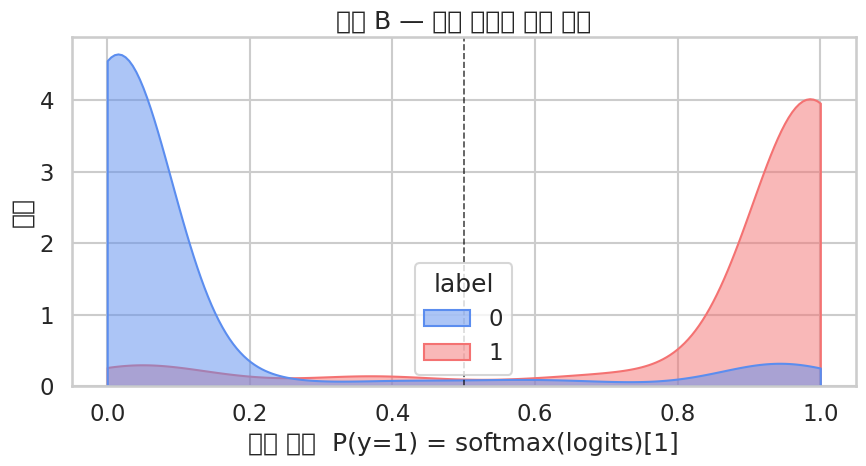
\includegraphics[width=0.88\linewidth]{assets/figures/ch11_probability_kde.png}
\end{bookfigurelabel}



\subsection{\texorpdfstring{로짓 차이 분포}{z = z\_1 - z\_0 의 logit 공간 분포}}

방식 B는 logit이 2차원 \((z_0, z_1)\) 이라 단순한 logit 공간 그림이 안 그려집니다. 그래서 \textbf{방식 A와 같은 1차원 logit 좌표로 환산} (\(z = z_1 - z_0\)) 해서 그립니다 --- 이러면 결정 경계는 \(z=0\), 의미는 \(\sigma(z)=p_1\) 로 방식 A와 정확히 같아집니다.



\Needspace{16\baselineskip}
\begin{lstlisting}
fig, ax = plt.subplots(figsize=(9, 5))
sns.kdeplot(
    data=df, x="logit", hue="label",
    fill=True, common_norm=False, alpha=0.5,
    palette=PAL, ax=ax,
)
ax.axvline(0.0, color="black", lw=1.2, ls="--", alpha=0.7)
ax.set_title("Method B — Logit Distribution  (z = z1 − z0)")
ax.set_xlabel("Logit  z = z1 − z0")
ax.set_ylabel("Density")
plt.tight_layout()
plt.show()
\end{lstlisting}

\begin{bookfigurelabel}[htbp]{방식 B를 1차원 logit 차이로 환산한 분포}{fig:ch11-logit-kde}
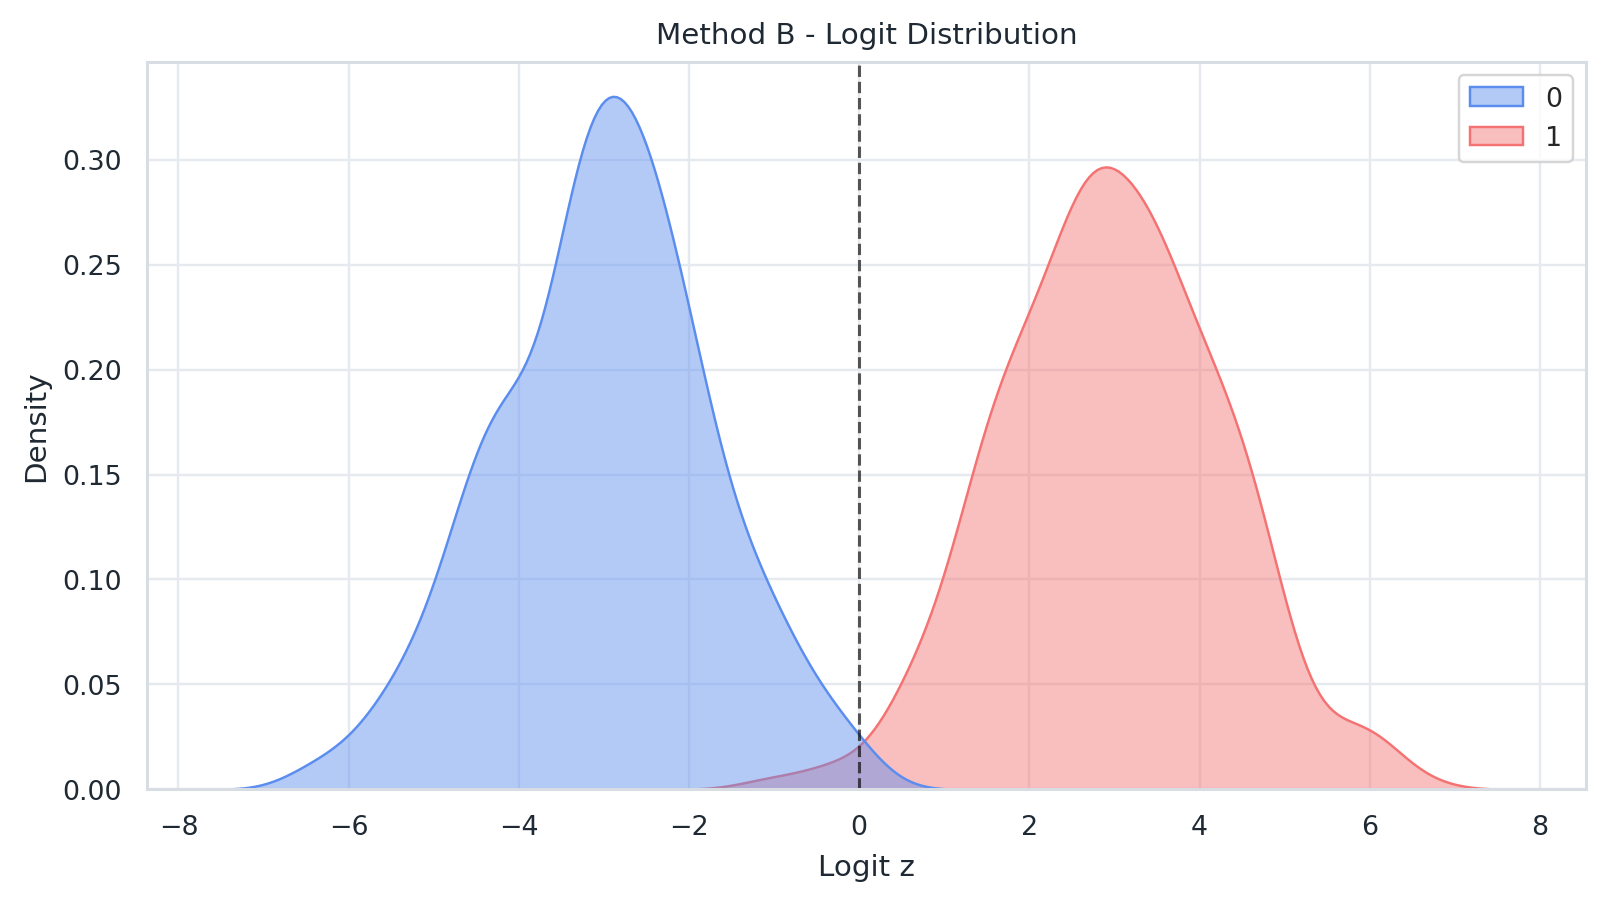
\includegraphics[width=0.88\linewidth]{assets/figures/ch11_logit_kde.png}
\end{bookfigurelabel}



\textbf{여기까지 정리} --- 4-1과 4-2의 그림은 \ref{ch:10}장의 것과 \emph{모양} 이 거의 같아야 합니다. 봉우리 높이나 위치가 미세하게 다를 순 있어도, 양 끝 압착 / 가운데 혼동 영역 / 결정 경계 자리 같은 \emph{큰 그림} 은 동일. 이게 두 방식 동등성의 \emph{시각적} 증거.



\Needspace{9\baselineskip}
\begin{lstlisting}
print(classification_report(
    labels, probs_full.argmax(axis=1),
    target_names=["negative", "positive"],
    digits=4,
))
\end{lstlisting}



\section{\texorpdfstring{방식 A/B 비교}{방식 A/B 비교}}

이전 장(\ref{ch:10}장)의 결과 파일에 의존하지 않도록, 같은 데이터·같은 hyperparams·같은 seed로 방식 A를 \emph{바로 여기서} 한 번 더 학습합니다. 변하는 것은 \textbf{모델 셋업과 라벨 형식뿐} (\ref{ch:10}장에서 본 그대로):

\begin{booktable}{11장 방식 A/B 비교 표}{tab:ch11-05}
\begin{adjustbox}{max width=\textwidth}
\begin{tabular}{@{}lll@{}}
\toprule
셋업 & 방식 B (§3-4에서 학습) & 방식 A (지금 inline 재학습) \\
\midrule

\inlinecode{num\_labels} & 2 & \textbf{1} \\
\inlinecode{problem\_type} & \inlinecode{single\_label\_classification} & \textbf{\inlinecode{multi\_label\_classification}} \\
라벨 형식 & int 스칼라 (\inlinecode{0} / \inlinecode{1}) & \textbf{길이 1 multi-hot float (\texttt{{[}0.0{]}} / \texttt{{[}1.0{]}})} \\
학습 hyperparams & (epoch=2, lr=2e-5, seed=42 \ldots) & \textbf{그대로} \\
\bottomrule
\end{tabular}
\end{adjustbox}
\end{booktable}

T4 기준 추가 \textasciitilde8분. 학습이 끝나면 같은 eval 셋의 \(p_A^{(i)}\) 와 §4에서 구한 \(p_B^{(i)}\) 를 1,000개 점으로 비교할 수 있게 됩니다.



\Needspace{25\baselineskip}
\begin{lstlisting}
def to_method_a_labels(batch):
    batch["labels"] = [[float(l)] for l in batch["labels"]]
    return batch

train_tok_A = train_tok.map(
    to_method_a_labels,
    batched=True,
)
eval_tok_A  = eval_tok.map(
    to_method_a_labels,
    batched=True,
)

print(
    f"Method A first sample label: "
    f"{train_tok_A[0]['labels']}  (length-1 float vector)"
)
print(
    f"Method B first sample label: "
    f"{train_tok[0]['labels']}    (int scalar)"
)
\end{lstlisting}



\Needspace{26\baselineskip}
\begin{lstlisting}
model_A = AutoModelForSequenceClassification.from_pretrained(
    "distilbert-base-uncased",
    num_labels=1,
    problem_type="multi_label_classification",
)

def compute_metrics_A(eval_pred):
    logits, lbl = eval_pred
    logits = logits.flatten()
    lbl    = lbl.flatten().astype(int)
    p_hat  = 1.0 / (1.0 + np.exp(-logits))
    preds  = (p_hat >= 0.5).astype(int)
    p, r, f1, _ = precision_recall_fscore_support(
        lbl,
        preds,
        average="binary",
        zero_division=0,
    )
    return {
        "accuracy":  float(accuracy_score(lbl, preds)),
        "precision": float(p),
        "recall":    float(r),
        "f1":        float(f1),
        "auc":       float(roc_auc_score(lbl, p_hat)),
    }

print(f"Method A classifier:    {model_A.classifier}")
print(
    f"Method A problem_type:  "
    f"{model_A.config.problem_type}"
)
\end{lstlisting}



\Needspace{26\baselineskip}
\begin{lstlisting}
training_args_A = TrainingArguments(
    output_dir="./ch11_method_a_output",
    num_train_epochs=2,
    per_device_train_batch_size=16,
    per_device_eval_batch_size=32,
    learning_rate=2e-5,
    fp16=True,
    eval_strategy="epoch",
    logging_steps=50,
    save_strategy="no",
    report_to="none",
    seed=42,
)

trainer_A = Trainer(
    model=model_A,
    args=training_args_A,
    train_dataset=train_tok_A,
    eval_dataset=eval_tok_A,
    processing_class=tokenizer,
    compute_metrics=compute_metrics_A,
)

train_result_A = trainer_A.train()
print(
    f"\nMethod A training done — train loss: "
    f"{train_result_A.training_loss:.4f}"
)
\end{lstlisting}



\Needspace{16\baselineskip}
\begin{lstlisting}
preds_A_out = trainer_A.predict(eval_tok_A)
logits_A    = preds_A_out.predictions.flatten()
probs_A     = 1.0 / (1.0 + np.exp(-logits_A))
labels_A    = preds_A_out.label_ids.flatten().astype(int)

assert (labels_A == labels).all(), "Sample order mismatch — check eval_tok / eval_tok_A derivation"

eval_metrics_A = trainer_A.evaluate()
print("Method A evaluation:")
for k, v in eval_metrics_A.items():
    if k.startswith("eval_") and isinstance(v, float):
        print(f"  {k:>20}: {v:.4f}")
\end{lstlisting}



\subsection{평가지표 비교}

같은 데이터에 같은 모델 본체로 학습했고 hyperparams도 같으니, accuracy/F1/AUC 같은 평가 지표가 \emph{거의 같은} 값이어야 합니다. 차이가 있다면 random init과 dropout 같은 \emph{학습 경로} 차이에서 옵니다.



\Needspace{25\baselineskip}
\begin{lstlisting}
metrics_A = {k.replace(
    "eval_",
    ""): v for k,
    v in eval_metrics_A.items(,
)
             if k.startswith("eval_") and isinstance(v, float)}
metrics_B = {k.replace(
    "eval_",
    ""): v for k,
    v in eval_metrics.items(,
)
             if k.startswith("eval_") and isinstance(v, float)}

common = [k for k in metrics_A if k in metrics_B]
cmp = pd.DataFrame({
    "metric":                  common,
    "method A (sigmoid+BCE)":  [metrics_A[k] for k in common],
    "method B (softmax+CE)":   [metrics_B[k] for k in common],
})
cmp["|A-B|"] = (cmp["method A (sigmoid+BCE)"] - cmp["method B (softmax+CE)"]).abs()
print(cmp.round(4).to_string(index=False))
\end{lstlisting}



\subsection{확률 산점도}

x축 = 방식 A의 \(p_A\), y축 = 방식 B의 \(p_B\). 점 색은 정답 라벨.

\textbf{완전히 동등하면 모든 점이 \(y = x\) 직선 위}. 실제로는 random init·dropout·optimizer 비결정성 때문에 약간 흩어지지만, 직선에서 크게 벗어나면 안 됩니다.



\Needspace{26\baselineskip}
\begin{lstlisting}
df_cmp = pd.DataFrame({
    "prob_A": probs_A,
    "prob_B": probs,
    "label":  labels.astype(int),
})

fig, ax = plt.subplots(figsize=(7, 7))
sns.scatterplot(
    data=df_cmp, x="prob_A", y="prob_B", hue="label",
    palette={0: "#5B8DEF", 1: "#F47272"}, alpha=0.55, s=35, ax=ax,
)
ax.plot([0, 1], [0, 1], color="black", lw=1.3, ls="--", alpha=0.7,
        label="y = x (perfect equivalence)")
ax.set_xlim(-0.02, 1.02); ax.set_ylim(-0.02, 1.02)
ax.set_xlabel("Method A — P(y=1) = sigmoid(z_A)")
ax.set_ylabel("Method B — P(y=1) = softmax(z_0, z_1)[1]")
ax.set_title("Method A vs Method B — per-sample probability agreement")
ax.legend(loc="upper left")
plt.tight_layout()
plt.show()

corr = float(np.corrcoef(probs_A, probs)[0, 1])
mae  = float(np.abs(probs_A - probs).mean())
print(
    f"Pearson corr:        "
    f"{corr:.4f}  (1.0 = perfect equivalence)"
)
print(f"Mean abs diff |A-B|: {mae:.4f}")
\end{lstlisting}

\begin{bookfigurelabel}[htbp]{방식 A와 방식 B의 샘플별 확률 일치도}{fig:ch11-probability-scatter}
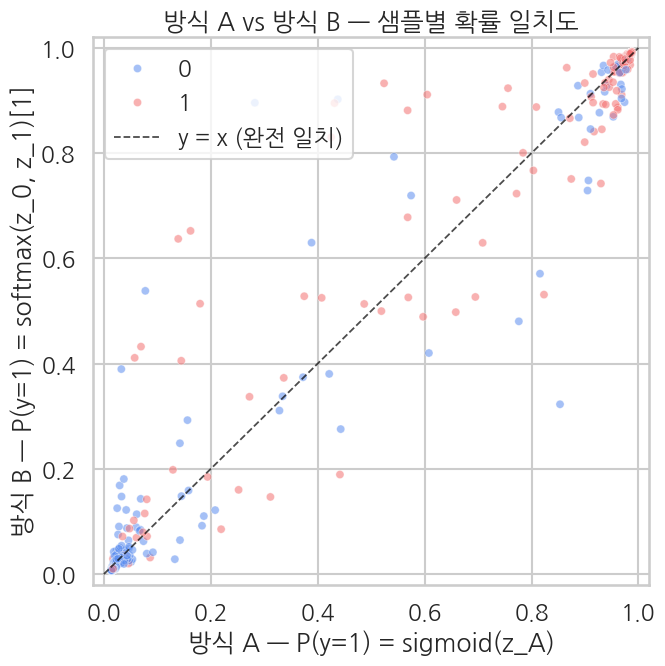
\includegraphics[width=0.72\linewidth]{assets/figures/ch11_probability_scatter.png}
\end{bookfigurelabel}



\textbf{해석}

\begin{itemize}
\tightlist
\item
  \textbf{상관계수가 0.99 이상}, \textbf{평균 절대 차가 0.05 이하} 면 두 방식이 사실상 같은 함수를 학습했다고 봐도 됩니다.
\item
  만약 점들이 \emph{체계적으로} 직선 한쪽으로 치우친다면 → 한 방식이 다른 방식보다 일관되게 더 자신 있게 / 더 보수적으로 예측하고 있다는 뜻. seed를 여러 개 시도해 평균내면 보통 사라집니다.
\item
  점들이 직선 \emph{주변에 무작위로} 흩어져 있으면 → 단순 학습 경로 차이. 학습량을 늘리거나 더 큰 데이터에서 학습하면 줄어듭니다.
\end{itemize}



\subsection{예측 일치율}

확률을 0/1 예측으로 떨어뜨린 뒤 두 방식의 예측이 얼마나 일치하는지 봅니다. 일치율이 95\% 이상이면 \emph{실질적으로} 같은 분류기로 봐도 됩니다.



\Needspace{20\baselineskip}
\begin{lstlisting}
pred_A = (probs_A >= 0.5).astype(int)
pred_B = (probs   >= 0.5).astype(int)

agree         = (pred_A == pred_B).mean()
both_correct  = ((pred_A == labels) & (pred_B == labels)).mean()
only_A_right  = ((pred_A == labels) & (pred_B != labels)).mean()
only_B_right  = ((pred_A != labels) & (pred_B == labels)).mean()
both_wrong    = ((pred_A != labels) & (pred_B != labels)).mean()

print(f"Agreement rate (A vs B predictions): {agree:.1%}")
print()
print(f"Prediction quadrants:")
print(f"  both correct:           {both_correct:.1%}")
print(f"  only A correct (B wrong): {only_A_right:.1%}")
print(f"  only B correct (A wrong): {only_B_right:.1%}")
print(f"  both wrong:             {both_wrong:.1%}")
\end{lstlisting}



\textbf{여기까지 보고 결론} --- 식으로 본 동등성 (\(\sigma(z) = \mathrm{softmax}(z_0, z_1)[1]\) when \(z = z_1 - z_0\))이 BERT에서도 그대로 성립합니다. 차이가 있어 봐야 random init / dropout 같은 \emph{학습 경로 차이} 정도. 두 방식은 \textbf{수식이 다른 같은 모델}, 라이브러리·코드 컨벤션이 강요하는 표현 차이일 뿐입니다.

\begin{quote}
\textbf{현장 가이드}: 새 BERT 분류 task를 시작할 때는 \emph{방식 B (softmax+CE)} 가 표준 --- \inlinecode{num\_labels=K}, \inlinecode{problem\_type="single\_label\_classification"} 만 두면 끝. 방식 A는 \emph{binary 라벨이 multi-label 형식으로 들어오는 시나리오} (예: 이진 라벨이 여러 헤드 중 하나로 끼어 있는 경우)에서만 의식적으로 사용합니다.
\end{quote}



\section{이 장에 등장한 라이브러리·함수}

\begin{booktable}{11장 새로 등장한 라이브러리}{tab:ch11-06}
\begin{adjustbox}{max width=\textwidth}
\begin{tabular}{@{}lll@{}}
\toprule
이름 & 한 줄 설명 & 다음 장에서 \\
\midrule

\inlinecode{AutoModelForSequenceClassification(num\_labels=2,\ problem\_type="single\_label\_classification")} & BERT 표준 분류 셋업 & \ref{ch:12}장 (multi-class)에서 \inlinecode{num\_labels=5} 만 바꿔 그대로 \\
\inlinecode{id2label} / \inlinecode{label2id} & config에 사람이 읽는 라벨 이름 등록 (\ref{ch:07}장 appendix에서 본 것) & 분류 장마다 권장 \\
\inlinecode{numpy.exp\ /\ sum} 으로 직접 softmax & 안정 softmax 수동 구현 (\inlinecode{max} 빼고 정규화) & \ref{ch:12}·\ref{ch:13}장에서 multi-class 확률 추출에 동일 패턴 \\
\inlinecode{seaborn.scatterplot(hue=,\ alpha=)} & 두 모델의 sample-level prediction 비교에 적합 & \ref{ch:14}장 auxiliary loss 비교에서 다시 사용 \\
\inlinecode{numpy.corrcoef}, \inlinecode{numpy.abs(a-b).mean()} & 두 분포의 동등성을 수치로 정량화 & 모델 비교가 필요한 장마다 \\
\bottomrule
\end{tabular}
\end{adjustbox}
\end{booktable}



\section{체크포인트 질문}

\begin{enumerate}
\def\labelenumi{\arabic{enumi}.}
\tightlist
\item
  방식 B의 출력 logit shape이 \inlinecode{(B,\ 2)} 인데, 방식 A와 비교할 1차원 logit을 어떻게 만드나요? 왜 그게 정당한가요?
\item
  \inlinecode{problem\_type="single\_label\_classification"} 과 \inlinecode{"multi\_label\_classification"} 의 차이를 한 줄로 설명한다면?
\item
  방식 A와 방식 B의 \emph{학습된 가중치} 가 똑같지 않은데도 \emph{최종 확률} 이 거의 같은 이유는?
\item
  scatter plot에서 점들이 \(y=x\) 직선에서 \emph{체계적으로} 위 또는 아래로 치우친다면 무엇을 의심해야 하나요?
\end{enumerate}



\section{FAQ}

\begin{faqBox}{Q1. (실무) BERT 이진 분류는 단순히 방식 B 쓰면 되는 거죠?}

네, 99\%의 경우 방식 B가 답입니다.

\Needspace{9\baselineskip}
\begin{lstlisting}
model = AutoModelForSequenceClassification.from_pretrained(
    "bert-base-uncased",
    num_labels=2,
    problem_type="single_label_classification",
)
\end{lstlisting}

방식 A는 \emph{이진 라벨이 multi-label 형식으로 들어와야 하는 특수 시나리오} (예: K개 라벨 중 하나만 binary로 처리하고 나머지는 다른 헤드에 붙이는 구조)에서만 의식적으로 씁니다. 일반 binary classification은 단순히 B.

\end{faqBox}

\begin{faqBox}{Q2. (이론) \ref{ch:04}장의 sklearn 동등성 시연(\inlinecode{predict\_proba} 일치)과 \ref{ch:11}장의 BERT 동등성 시연(scatter plot) 의 차이는?}

\begin{booktable}{11장 FAQ 표}{tab:ch11-07}
\begin{adjustbox}{max width=\textwidth}
\begin{tabular}{@{}lll@{}}
\toprule
& \ref{ch:04}장 (sklearn) & \ref{ch:11}장 (BERT) \\
\midrule

두 모델이 \emph{같은 가중치} 를 학습? & \textbf{사실상 그렇다} --- 작은 모델이라 두 방식이 같은 최적해로 수렴 & 아니다 --- 67M 파라미터 중 일부가 random init 차이로 다른 곳에 정착 \\
\inlinecode{predict\_proba} 가 정확히 같은가? & \textbf{거의 일치} (소수점 4-5자리까지) & \emph{근사적으로} 일치 (Pearson 0.99+, MAE 0.01-0.05) \\
차이의 출처 & sklearn 옵티마이저 수렴 정밀도 & random init + dropout + GPU 비결정성 \\
\bottomrule
\end{tabular}
\end{adjustbox}
\end{booktable}

수학적 동등성(\(\sigma(z) = \mathrm{softmax}(z_0,z_1)[1]\) where \(z=z_1-z_0\))은 두 경우 모두 성립합니다. 구현 차원의 노이즈 양이 다를 뿐.

\end{faqBox}

\begin{faqBox}{Q3. (실무) \inlinecode{compute\_metrics} 안의 softmax를 직접 구현하지 말고 \inlinecode{torch.softmax} 쓰면 안 되나요?}

써도 됩니다. 단, \inlinecode{compute\_metrics} 가 받는 \inlinecode{logits} 는 \emph{numpy 배열} 이라 \inlinecode{torch.from\_numpy} 로 한 번 감싸야 합니다.

\Needspace{9\baselineskip}
\begin{lstlisting}
import torch
probs_full = torch.softmax(
    torch.from_numpy(logits),
    dim=-1).numpy(,
)
\end{lstlisting}

이 장에선 \emph{softmax가 어떻게 동작하는지} 노출하기 위해 \inlinecode{np.exp\ /\ sum} 으로 직접 짰습니다 --- \inlinecode{max} 빼서 안정화하는 부분이 곧 PyTorch 내부 구현과 동일한 트릭입니다.

\end{faqBox}

\begin{faqBox}{Q4. (이론) 방식 A는 sklearn \inlinecode{LogisticRegression()} 과 같은 셋업이고, 방식 B는 \inlinecode{LogisticRegression(multi\_class="multinomial")} 같은 셋업이라고 했는데 --- 그러면 sklearn에서도 두 모델의 학습 결과가 BERT처럼 다른가요?}

sklearn에서는 두 \emph{방식} 의 차이가 BERT보다 훨씬 작습니다. 이유는:

\begin{enumerate}
\def\labelenumi{\arabic{enumi}.}
\tightlist
\item
  \textbf{모델 크기}: sklearn LogReg는 \textasciitilde10K 파라미터. BERT는 67M. 작은 모델이 큰 모델보다 \emph{유일한 최적해} 로 수렴하기 쉽습니다.
\item
  \textbf{무작위성 원천}: sklearn LogReg는 \inlinecode{liblinear}/\inlinecode{lbfgs} 같은 결정론적 옵티마이저 기본. BERT는 SGD 기반 + GPU + dropout 으로 \emph{원천적으로} 비결정적.
\item
  \textbf{데이터 표현}: sklearn TF-IDF는 sparse fixed feature. BERT는 매 backprop마다 hidden state도 업데이트.
\end{enumerate}

그래서 \ref{ch:04}장에서는 두 sklearn 모델의 \inlinecode{predict\_proba} 가 \emph{소수점 4-5 자리} 까지 같았고, \ref{ch:11}장에서는 \emph{소수점 1-2 자리} 수준에서 같습니다.

\end{faqBox}

\begin{faqBox}{Q5. (실무) 학습된 모델을 저장·로드할 때 두 방식 모델은 호환되나요?}

\textbf{아니요, 분류 헤드 shape이 달라서 직접 호환되지 않습니다.}

\begin{itemize}
\tightlist
\item
  방식 A: \inlinecode{classifier.weight.shape\ =\ (1,\ 768)}, \inlinecode{classifier.bias.shape\ =\ (1,)}
\item
  방식 B: \inlinecode{classifier.weight.shape\ =\ (2,\ 768)}, \inlinecode{classifier.bias.shape\ =\ (2,)}
\end{itemize}

\inlinecode{from\_pretrained} 로 다른 방식의 체크포인트를 로드하면 분류 헤드를 \emph{새로 초기화} 한다는 경고가 뜹니다 (DistilBERT body는 그대로 로드됨). 따라서 두 방식 사이의 변환은 \emph{처음부터 다시 학습} 이 정확합니다.

만약 \textbf{같은 표현력을 유지하면서} 변환하고 싶다면, 방식 A의 \(w_A, b_A\) 로부터 방식 B의 헤드를 다음과 같이 만들 수 있습니다 --- 한쪽 클래스 logit을 0으로 고정하면 됩니다.

\Needspace{12\baselineskip}
\begin{lstlisting}
W_A = model_A.classifier.weight    # shape (1, 768)
b_A = model_A.classifier.bias      # shape (1,)

W_B = torch.cat([torch.zeros_like(W_A), W_A], dim=0)
b_B = torch.cat(
    [torch.zeros_like(b_A), b_A],
    dim=0)  # (2,,
)
\end{lstlisting}

이러면 \(z_1 - z_0 = (W_A x + b_A) - 0 = z_A\) 가 정확히 일치합니다. 실무에선 거의 안 쓰지만 \emph{수학적 동등성} 의 구체적 모습을 보여주는 좋은 예시.

\end{faqBox}

\begin{faqBox}{Q6. (실무) \inlinecode{id2label} / \inlinecode{label2id} 는 꼭 등록해야 하나요?}

학습·평가 자체에는 영향 없지만 \textbf{추론 시 편리} 합니다.

\Needspace{10\baselineskip}
\begin{lstlisting}
pipe = pipeline(
    "text-classification",
    model=model,
    tokenizer=tokenizer,
)
pipe("Great food!")
\end{lstlisting}

또 \inlinecode{model.config.id2label} 이 huggingface hub에 모델을 올릴 때 widget 라벨 표시용으로 쓰입니다. 한 줄 추가로 큰 이득이라 항상 등록하는 게 좋습니다.
\end{faqBox}



\section{오류 실험 (선택)}

다음 코드를 돌려보면 어떤 에러가 날까요?

\Needspace{12\baselineskip}
\begin{lstlisting}
def tokenize_wrong(batch):
    out = tokenizer(
        batch["text"],
        truncation=True,
        max_length=128,
    )
    out["labels"] = [[float(b)] for b in batch["binary"]]
    return out
\end{lstlisting}

힌트: \inlinecode{CrossEntropyLoss} 가 받는 라벨은 \emph{int 인덱스 텐서} (shape \inlinecode{(B,)})인데 위 코드는 \emph{float 2차원 텐서} (shape \inlinecode{(B,\ 1)})을 넘깁니다. 텐서 dtype과 shape을 동시에 틀린 케이스라 메시지가 다소 길게 나올 수 있습니다.



\begin{previewBox}{미리보기: 다음 장}

\textbf{\ref{ch:12}장. BERT 다중 클래스 분류 (Multi-class \& CE)}

\begin{itemize}
\tightlist
\item
  Yelp 별점 1-5 를 그대로 5클래스 분류로 (\ref{ch:05}장의 sklearn 버전을 BERT로)
\item
  \inlinecode{num\_labels=5}, \inlinecode{problem\_type="single\_label\_classification"} (\ref{ch:11}장과 같은 표준 셋업, K만 2 → 5)
\item
  Activation은 그대로 softmax, Loss는 그대로 \inlinecode{CrossEntropyLoss}
\item
  \textbf{변하는 축은 \emph{task} 하나} --- Loss·activation·문제 셋업이 동일. K=2가 K=5로 자연스럽게 일반화되는 모습 확인
\end{itemize}

\begin{quote}
\textbf{Phase 1 흐름 정리 (\ref{ch:07}장 - \ref{ch:14}장)}: BERT (영어) 위에서 Regression(9) → Binary 방식 A(10) → Binary 방식 B(11) → Multi-class(12) → Multi-label(13) → Auxiliary(14). 한 장에 한 축씩만 변합니다.
\end{quote}
\end{previewBox}
